% Created 2016-04-06 Wed 14:25
\documentclass[10pt,t,a4paper]{beamer}
\usepackage[utf8]{inputenc}
\usepackage[T1]{fontenc}
\usepackage{fixltx2e}
\usepackage{graphicx}
\usepackage{longtable}
\usepackage{float}
\usepackage{wrapfig}
\usepackage{rotating}
\usepackage[normalem]{ulem}
\usepackage{amsmath}
\usepackage{textcomp}
\usepackage{marvosym}
\usepackage{wasysym}
\usepackage{amssymb}
\usepackage{hyperref}
\tolerance=1000
\usetheme{BTH_msv}
\author{Mikael Svahnberg\thanks{Mikael.Svahnberg@bth.se}}
\date{2016-04-06}
\title{Modelling Behaviour \\\\ \texttt{PA14[13]5}}
\hypersetup{
  pdfkeywords={},
  pdfsubject={},
  pdfcreator={Emacs 25.1.50.1 (Org mode 8.2.10)}}
\begin{document}

\maketitle

\section{Classroom}
\label{sec-1}
\begin{frame}[shrink=25,label=sec-1-1]{Example: \\ From Use Case to Sequence Diagram}
\begin{center}
\begin{tabular}{p{7cm}p{7cm}}
Actor Action & System Response\\
\hline
1. Customer arrives at a checkout with items to purchase & \\
2. Cashier records identifier from each item & 3. Determines item price and adds item info to running sale transaction. Description and price of current item are presented.\\
4. On completion of item entry, Cashier indicates to PoS that item entry is complete & 5. Calculates and presents the sale total.\\
6. Cashier tells Customer the total. & \\
7. Customer gives cash to Cashier. & \\
8. Cashier records received cash & 9. Shows the balance due to the Customer\\
 & 10. Prints receipt\\
11. Cashier deposits the cash and extracts the balance. & \\
 & 12. Logs the complete sale\\
 & \\
13. C gives printed receipt to B with balance & \\
14. B leaves with the items and recept. & \\
\hline
\end{tabular}
\end{center}
\end{frame}
\begin{frame}[label=sec-1-2]{More on Sequence Diagrams}
\vspace{-1cm}\hspace{2cm}
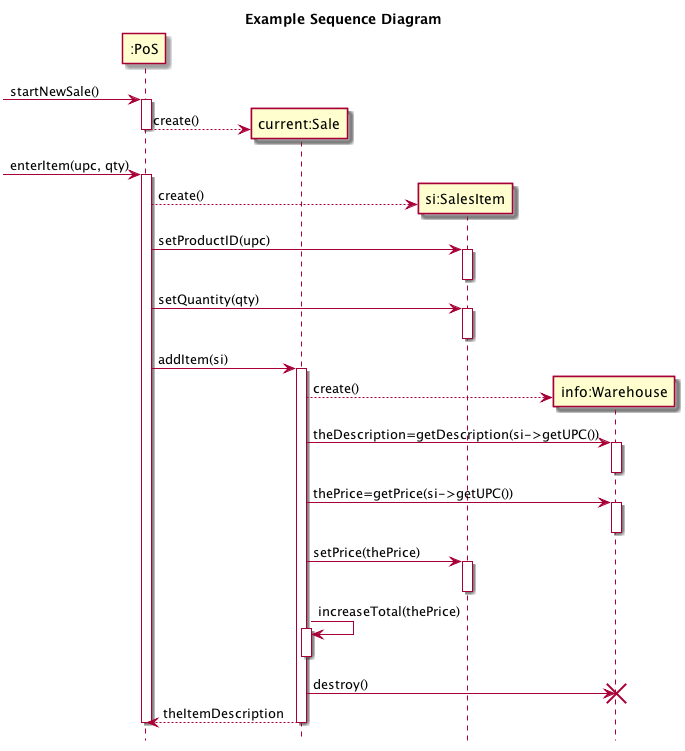
\includegraphics[height=8cm]{FSequenceDiagrams.png}
\end{frame}

\begin{frame}[label=sec-1-3]{Communication Diagrams \\ (Interaction Diagrams)}
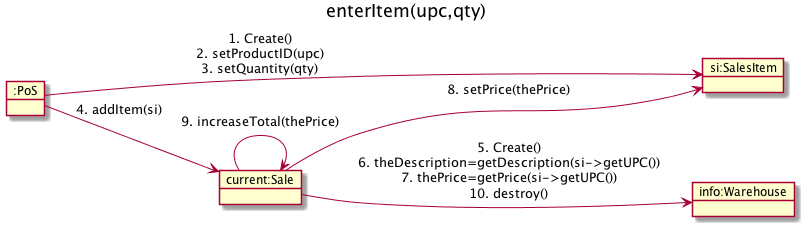
\includegraphics[width=10cm]{FCommunicationDiagram.png}
\end{frame}

\begin{frame}[label=sec-1-4]{Discuss: Contracts}
\begin{itemize}
\item What are contracts?
\begin{itemize}
\item Why are we writing them?
\end{itemize}
\item How should you interpret preconditions?
\item How to interpret postconditions?
\item What are their relation to Sequence Diagrams, Class Diagrams?
\item What are extended contracts good for?
\begin{itemize}
\item When might you need Extended Contracts?
\end{itemize}
\end{itemize}
\end{frame}
\begin{frame}[label=sec-1-5]{State Diagrams}
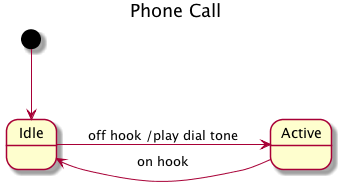
\includegraphics[width=.9\linewidth]{FStateDiagramExample4.png}
\end{frame}

\begin{frame}[label=sec-1-6]{Nested States}
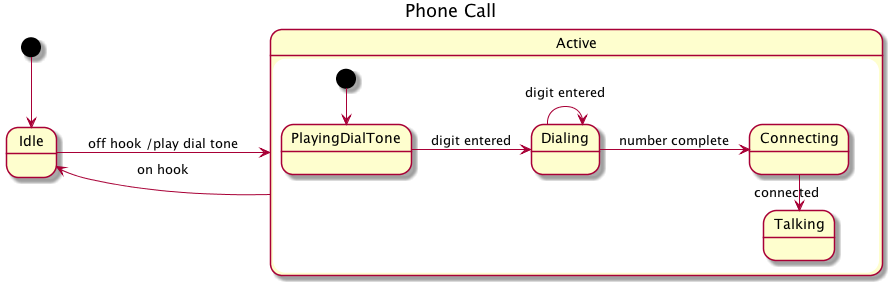
\includegraphics[width=.9\linewidth]{FStateDiagramExamplePhoneNested.png}
\end{frame}

\begin{frame}[label=sec-1-7]{Discuss: State Diagrams}
\begin{itemize}
\item What is a State?
\begin{itemize}
\item When is it meaningful to model states?
\end{itemize}
\item What is an Action and what is a State Change?
\begin{itemize}
\item Also discuss this for Contracts
\end{itemize}
\item How can we use state diagrams in the context of UML to avoid extra work?
\end{itemize}
\end{frame}
\begin{frame}[label=sec-1-8]{Example State Diagram (bad)}
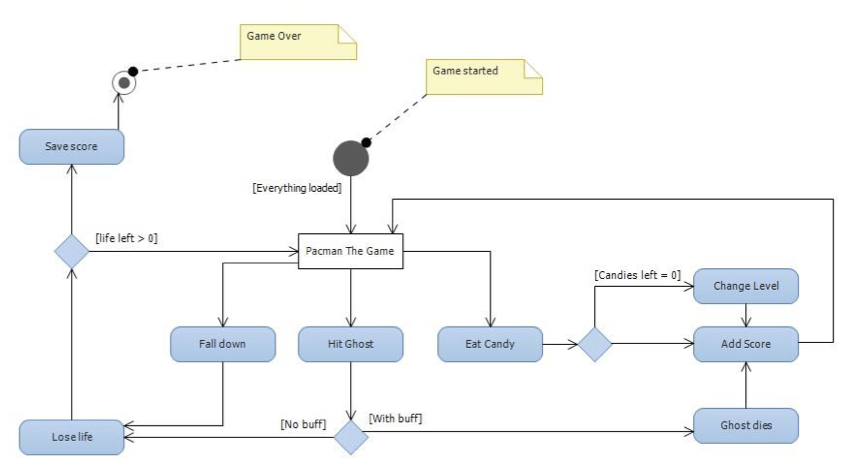
\includegraphics[width=11cm]{./FExampleBadStateChart.png}
\end{frame}
\begin{frame}[label=sec-1-9]{Example State Diagram (better)}
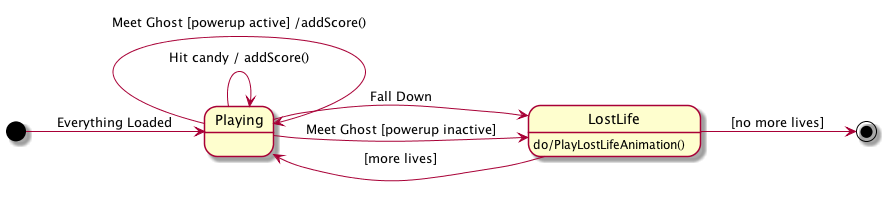
\includegraphics[width=11cm]{FExampleBadStateChart_fixed.png}
\end{frame}
\begin{frame}[label=sec-1-10]{Discussion: Dynamic Behaviour}
\begin{itemize}
\item Why should we model the behaviour?
\end{itemize}
\end{frame}
% Emacs 25.1.50.1 (Org mode 8.2.10)
\end{document}